\chapter{Materials and methods}

\section{Datasets}

  Six datasets have been used in the framework of this thesis:
  one for training the model, one for optimizing the hyper-parameters, and four for benchmarking.
  The training and validation sets together compose the 180 protein families used by Michel and Skwark~\cite{Skwark079673}.
  These 180 families comprise the 150 protein families reported in the original
  PSICOV article~\cite{doi:10.1093/bioinformatics/btr638}, as well as 30 protein families selected from the test set of
  PConsC2~\cite{10.1371/journal.pcbi.1003889}.

  The first test set is composed of 210 proteins having no homology to the training set or the validation set.
  To achieve this goal, homology reduction has been applied to the 383 proteins used in the testing of PConsC2.
  This homology reduction was conducted by ensuring that no protein in the test set is assigned the same
  ECOD H-class~\cite{10.1371/journal.pcbi.1003926} as any protein from the training or validation set.

  Three additional test sets have also been considered in order to make a direct comparison with the state-of-the-art RaptorX-Contact predictor.
  Consequently, the second test set embodies the 105 protein domains from the CASP11 experiment, the third test set 76 proteins from the CAMEO
  project, and the fourth test set 398 membrane proteins.

  \todo{Profile HMMs: \cite{eddy1998profile}}
  MSAs have been created using HHblits~\cite{HHblits} (version as of the date of 26th February 2016) on the Uniprot20 database
  with an e-value of 1. Parameters have been set in such a way that all sequences in each of the database's MSA are aligned.
  The obtained MSAs have been used as input to all other predictors and intermediate predictors, allowing for easier comparability.

  All protein sequences, structures, MSAs and intermediate predictions used in this thesis come from the datasets that were publicly
  available at the address \url{http://pconsc3.bioinfo.se/pred/download/} as on the date of 28th December 2018.
  Information available in these datasets is the following:

  \todo{PDB parser to obtain distance and contact maps}

  \begin{itemize}
    \item Protein sequence in FASTA format
    \item MSA obtained using HHblits on the corresponding protein family
    \item Atom 3D coordinates
    \item PhyCMAP~\cite{PhyCMap} intermediate predictions
    \item plmDCA~\cite{EKEBERG2014341} intermediate predictions
    \item GaussDCA~\cite{10.1371/journal.pone.0092721} intermediate predictions
    \item Predictions made by PConsC3~\cite{Skwark079673} at each layer of the model
    \item CCMPred~\cite{CCMPred} predictions (only available in the 4 test sets)
    \item EVFold~\cite{Sheridan021022} predictions (only available in the 4 test sets)
    \item PSICOV~\cite{doi:10.1093/bioinformatics/btr638} predictions (only available in the 4 test sets)
    \item MetaPSICOV~\cite{MetaPSICOV} predictions (only available in the 4 test sets)
  \end{itemize}

  \todo{Took alignments from PConsC2 and PConsC3 -> model not influenced by the new releases of alignments tools}
  \todo{What about the protein structures?}

  \todo{Oversampling negative class: \cite{markowski2016oversampling}}

\section{Input features}

  As described in section \ref{inputfeatures}, input features can be split into three categories:
  global, 1-dimensional and 2-dimensional features.
  The proposed model takes as input the protein length, the effective number of sequences 
  in the corresponding MSA, position-specific statistics, residue pair-specific statistics
  and predictions made by PSICOV, plmDCA and GaussDCA.

  \begin{table}[H]
    \centering
    \begin{tabular}{|l|l|c|}
      \hline
      Category & Feature name & Dimensionality \\
      \hline
      \hline
      Global & Protein length $L$ & scalar \\
             & Effective number of sequences $M_{eff}$ & scalar \\
      \hline
      1-dimensional & One-hot-encoded sequence & $L \times \naatypes$ \\
                    & Self-information & $L \times \naatypes$ \\
                    & Partial entropy & $L \times 2 \cdot \naatypes$ \\
      \hline
      2-dimensional & Mutual information & $L \times L$ \\
                    & Normalized mutual information & $L \times L$ \\
                    & Cross-entropy & $L \times L$ \\
                    & PSICOV predictions & $L \times L$ \\
                    & GaussDCA predictions & $L \times L$ \\
                    & plmDCA predictions & $L \times L$ \\
      \hline
    \end{tabular}
    \captionof{table}{Input features of the proposed model.
      Global features are scalar values, whereas dimensional
      features are presented in the form of matrices of given shape.}
    \label{hyperparams}
  \end{table}

\section{Proposed architecture}

  \begin{figure}[H]
    \begin{center}
      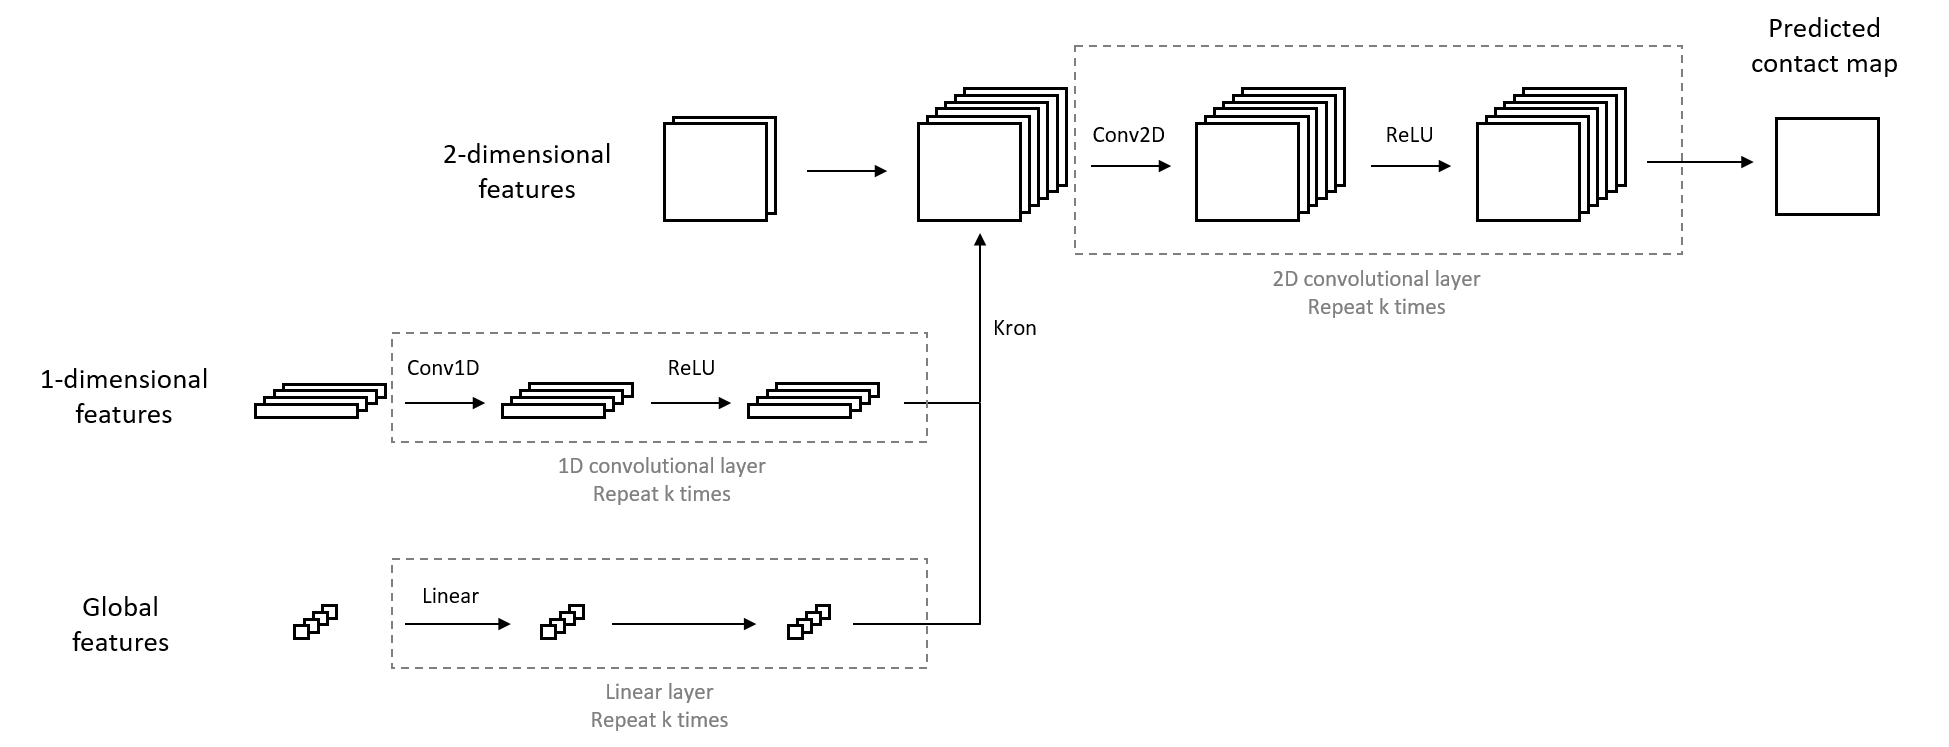
\includegraphics[width=\textwidth, keepaspectratio]{imgs/architecture.png}
       \caption{Proposed architecture of the deep convolutional neural network for semantic segmentation}
      \label{architecture}
    \end{center}
  \end{figure}

\section{Evaluation}

  Protein contact maps are imbalanced by nature: they contain very few residue contacts compared to their number of residue pairs.
  $L$ being the number of residues in a protein, the number of residue contacts increases linearly with $L$ while the number of residue pairs
  increases quadratically~\cite{OLMEA1997S25}. This is important because one can evaluate a model only on the $L$ (or even less than $L$) predicted
  residue contacts the model is the most confident about. Such evaluation metric is called \textit{best-L/k PPV (Positive Predictive Value)}
  and can be formulated as follows:

  \begin{equation}
    \text{Best-L/k PPV} = \frac{\sum_{\underset {i-j \geq 6}{(i, j) \in B(L/k)}} C_{i, j}}{L/k}
  \end{equation}

  where $C_{i, j}, N_{i, j} \in \{0, 1\} \ \forall i, j, i-j \ge 6$ are boolean values indicating a contact or a non-contact, respectively.
  $B(L/k)$ is the set of $L/k$ most confident predicted probabilities (with highest values) and $p_{i, j}$ is the predicted probability
  that residue pair $(i, j)$ forms a contact.
  Contacts under a residue distance of 6 amino acids are not considered during evaludation phase even though they are used during
  training phase.

  Best-L/k PPV can also be split into three separated metrics: short-range, medium-range and long-range contacts.
  These three types of contacts can be defined by the residue separations used by Skwark et al.~\cite{10.1371/journal.pcbi.1003889}:

    \begin{itemize}
      \item Short-range contacts: 6 - 12 residue separation
      \item Medium-range contacts: 12 - 24 residue separation
      \item Long-range contacts: 24+ residue separation
    \end{itemize}

\section{Hyper-parameter optimization}

  In order to ensure the best hyper-parameters are selected for the model that will be evaluated
  on the benchmark sets, the Hyperopt Python library~\cite{Bergstra_2015} has been used to explore
  the hyper-parameter space and fine-tune the model on the validation set.
  Training and evaluating a deep neural network is very costly and, as a matter of fact,
  each trial point in the hyper-parameter space should be carefully selected. Techniques based
  on grid search do not suit the problem because they are uninformed methods.

  Hyperopt provides an informed search method called Tree-structured Parzen Estimators (TPE)~\cite{bergstra2011algorithms}.
  In Bayesian hyper-optimization, the posterior probability $P(\alpha \vert L)$ is defined as a function
  of the hyper-parameter vector $\alpha$ and the loss $L$. Contrary to techniques based on Gaussian processes
  that approximates $P(\alpha \vert L)$ only, TPE models both posterior $P(\alpha \vert L)$ and $P(L)$.
  The prior is iteratively replaced with non-parametric densities based on generated points $\{ \alpha_1, \alpha_2, \dotsc \}$.
  It this search, TPE is an informed search strategy that refines its prior as new points are observed in the
  hyper-parameter space. The "tree structure" is due to the way the posterior is computed.

  \begin{equation}
    P(\alpha \vert L) =
      \begin{cases}
        l(\alpha) &  \text{if} \, L < L^* \\
        g(\alpha) &  \text{otherwise}
      \end{cases}
  \end{equation}

  Let $f$ be the prediction function of the model (see section \ref{backpropagation} about backpropagation algorithm),
  and let $f(\alpha) \triangleq \text{argmin}_{f(\Theta, \alpha)} c\big(f(\Theta, \alpha)\big)$ be the prediction function
  of a trained model that minimizes a given loss function $c$ w.r.t. a fixed hyper-parameter vector $\alpha$.
  $l(\alpha)$ is the non-parametric density function created by the observations $\{ \alpha^{i} \}$ such that
  $L = c(f(\alpha))$ is below the threshold $L^*$, and $g(\alpha)$ is created with the remaining observations.
  The threshold $L^*$ is set as a quantile of the observed values of $L$.
  The value to be optimized in TPE is the Expected Improvement (EI), which is measured as an infinitesimal sum
  of loss improvements weighted by the posterior. After applying Bayes formule to the posterior, calculus of EI becomes:

  \begin{equation}
    EI_{L^*}(\alpha) = \int_{-\infty}^{L^*} (L^* - L) P(L \vert \alpha) dL 
    = \int_{-\infty}^{L^*} (L^* - L) \frac{P(\alpha \vert L) P(L)}{P(\alpha)} dL
  \end{equation}

  In the framework of Adaptive Parzen Estimators, each hyper-parameter is associated a prior and a density function,
  and the estimator is built as a weighted mixture of them.
  For example, a continuous variable can be assigned:
  \begin{itemize}
    \item A uniform prior with lower bound $a$ and upper bound $b$.
    \item A function defined as a mixture of Gaussian distributions, each centered on a point of the hyper-parameter
    space. The standard deviation of a particular distribution can be set as the maximum between distances to the left and right
    neighbors.
  \end{itemize}

  The density function is either $l(\alpha)$ or $g(\alpha)$ depending on whether the loss function associated to current
  point is below the threshold or not.

  \begin{table}[H]
    \centering
    \begin{tabular}{|l|c|c|}
      \hline
      Module & Hyper-parameter & Set of values \\
      \hline
      \hline
      General & Batch size & $\{ 1, 2, 4, 8, 16, 32 \}$ \\
              & Batch normalization & $\{ \top, \bot \}$ \\
              & Track running state & $\{ \top, \bot \}$ \\
              & Learning rate & \text{TODO} \\
              & L2 penalty & \text{TODO} \\
              & Parameter optimization & $\{ \text{ADADELTA}, \text{Adagrad}, \text{Adam} \}$ \\
              & Activation function & $\{ \text{ReLU}, \text{ELU}, \text{LeakyReLU}, \text{Tanh} \}$ \\
              & Use global modules & $\{ \top, \bot \}$ \\
      \hline
      Global module & Depth & \{ 2, 3, 4, 5, 6, 7, 8, 9, 10 \} \\
      \hline
      1-dimensional module & Depth & $\{ 2, 3, 4, 5, 6, 7, 8, 9, 10 \}$ \\
                           & Filter size & $\{ 3, 5, 7 \}$ \\
                           & Number of filters & $\{ 8, 16, 32, 64 \}$ \\
      \hline
      2-dimensional module & Depth & $\{ 2, 3, 4, 5, 6, 7, 8, 9, 10 \}$ \\
                           & Filter size & $\{ 3, 5, 7 \}$ \\
                           & Number of filters & $\{ 8, 16, 32, 64 \}$ \\
      \hline
    \end{tabular}
    \captionof{table}{Hyper-parameter space for the proposed architecture.}
    \label{hyperparams}
  \end{table}

\section{Implementation}

  Torch~\cite{torch}
  Scikit-learn~\cite{scikit-learn}
  Cython~\cite{behnel2010cython}
